\documentclass[conference]{IEEEtran}

% ---------------- PACKAGES ----------------
\usepackage{graphicx}
\usepackage{amsmath}
\usepackage{cite}
\usepackage{url}
\usepackage{booktabs}
\usepackage{array}
\usepackage{float}
\usepackage{tikz}
\usepackage{hyperref}
\usepackage{xcolor}

\usetikzlibrary{positioning, arrows.meta, shapes.geometric}

\begin{document}

% ---------------- TITLE ----------------
\title{SentinelOps: Design and Implementation of a
Containerized Infrastructure Monitoring and
Automated Alerting Framework}

% ---------------- AUTHOR ----------------
\author{
\IEEEauthorblockN{Chethana Sri}
\IEEEauthorblockA{
Department of Computer Technology\\
Madras Institute of Technology, Anna University\\
Chennai, India\\
Email: chethanasriadusumalli@gmail.com
}
}

\maketitle

% ---------------- ABSTRACT ----------------
\begin{abstract}
Infrastructure monitoring is essential for maintaining the
availability, reliability, and performance of modern computing
systems. Manual monitoring and fragmented monitoring tools can
make it difficult to identify abnormal resource utilization and
respond to potential infrastructure failures. This paper presents
SentinelOps, a containerized infrastructure monitoring and
automated alerting framework developed using Prometheus,
Node Exporter, Grafana, Alertmanager, and Docker Compose.

The proposed framework collects system-level performance
metrics, including CPU utilization, memory consumption, disk
activity, network traffic, and system load. Prometheus periodically
scrapes and stores the collected metrics as time-series data,
while Grafana provides dashboards for visualizing system
performance. Configurable alerting rules are used to identify
critical resource conditions, and Alertmanager manages alert
grouping and routing. Docker Compose is used to simplify the
deployment and coordination of the monitoring components.

This paper presents the architecture, implementation, and
practical evaluation of SentinelOps through monitoring dashboards
and controlled alerting scenarios. The implementation demonstrates
how open-source monitoring technologies can be integrated into
a unified and reproducible infrastructure monitoring environment.
\end{abstract}

% ---------------- KEYWORDS ----------------
\begin{IEEEkeywords}
Infrastructure Monitoring, Observability, Prometheus,
Grafana, Node Exporter, Alertmanager, Docker,
Containerization, Automated Alerting
\end{IEEEkeywords}

% =================================================
% I. INTRODUCTION
% =================================================

\section{Introduction}

Modern computing environments depend on servers and distributed
infrastructure to support web applications, databases, cloud
services, and enterprise systems. The availability and performance
of these resources directly influence application reliability and
user experience. As infrastructure becomes increasingly complex,
continuous monitoring is essential for identifying resource
utilization patterns, detecting abnormal behaviour, and preventing
potential service disruptions.

Traditional approaches to infrastructure monitoring may involve
manually checking system resource usage or using separate tools
for collecting, visualizing, and managing monitoring information.
Such approaches can make it difficult for administrators to obtain
a unified view of system health. Delayed identification of issues
such as excessive CPU utilization, memory consumption, disk
capacity exhaustion, and unusual network activity can affect
system availability and operational efficiency.

Monitoring platforms provide mechanisms for collecting, storing,
querying, and visualizing system metrics. Prometheus is an
open-source monitoring and alerting toolkit that collects metrics
from configured targets and stores them as time-series data
\cite{prometheus}. Time-series management systems are specifically
designed to store and analyze continuously generated temporal data
\cite{jensen2017}. Node Exporter exposes hardware and operating
system metrics that can be collected by Prometheus
\cite{nodeexporter}. Grafana provides visualization capabilities
through customizable dashboards, allowing administrators to
interpret monitoring information effectively \cite{grafana}.

Although these technologies provide powerful individual
capabilities, integrating multiple monitoring components requires
careful configuration and coordination. Metric collection,
visualization, alert evaluation, and notification management must
work together to provide a practical monitoring solution.

To address this requirement, this paper presents SentinelOps,
a containerized infrastructure monitoring and automated alerting
framework developed by integrating Prometheus, Node Exporter,
Grafana, Alertmanager, and Docker Compose.

The system uses Node Exporter to expose host-level metrics, while
Prometheus periodically collects and stores these metrics. Grafana
dashboards present the collected information through visual panels
representing CPU utilization, memory usage, disk activity, network
traffic, system load, and process-related metrics. Prometheus
alerting rules evaluate predefined conditions and forward generated
alerts to Alertmanager, which manages alert grouping and routing
\cite{alerting,alertmanager}.

The monitoring components are deployed using Docker Compose,
which simplifies service configuration and coordinated deployment
\cite{dockercompose}.

The primary contributions of this work are:

\begin{itemize}
    \item Design and implementation of an integrated infrastructure
    monitoring framework using open-source technologies.

    \item Centralized collection and visualization of essential
    system-level performance metrics.

    \item Configuration of threshold-based alerting and alert
    routing for identifying critical infrastructure conditions.

    \item Containerized deployment of the monitoring stack using
    Docker Compose.

    \item Practical evaluation through monitoring dashboards and
    controlled alerting scenarios.
\end{itemize}

The remainder of this paper is organized as follows.
Section II discusses related technologies and monitoring
approaches. Section III presents the problem statement and
objectives. Section IV describes the proposed SentinelOps
architecture. Section V explains the system design and
implementation. Section VI presents the experimental setup.
Section VII discusses the observations and results. Section VIII
describes limitations and future enhancements, followed by
the conclusion in Section IX.

% =================================================
% II. RELATED WORK
% =================================================

\section{Related Work}

Infrastructure monitoring has evolved from basic system-level
resource inspection to integrated observability platforms capable
of collecting and analyzing operational data across distributed
environments. Existing research has examined the challenges of
monitoring cloud-native systems, containerized workloads, and
microservice-based applications.

Usman et al. presented a survey of observability in distributed
edge and container-based microservices \cite{usman2022}. Their
study discusses the growing complexity of distributed
infrastructures and the need for telemetry-based approaches
to improve system visibility, fault diagnosis, and operational
management. This work provides a broader research context for
monitoring frameworks that integrate infrastructure-level
metrics and observability components.

Giamattei et al. conducted a systematic grey literature review
of monitoring tools used in DevOps and microservice environments
\cite{giamattei2024}. Their study examined 71 monitoring tools
and compared their features, assumptions, constraints, and
supported monitoring information. The review highlights the
range of monitoring capabilities available to practitioners
and the challenge of selecting and integrating suitable tools
for a particular environment.

Time-series data management is another important area in
infrastructure monitoring. Jensen et al. surveyed time-series
management systems and discussed their architectures,
storage capabilities, and query-processing approaches
\cite{jensen2017}. Since monitoring platforms continuously
generate timestamped measurements, efficient storage and
analysis of time-series data form an important foundation
for metric-based monitoring.

Prometheus provides a time-series monitoring system that
collects metrics from configured targets using a pull-based
scraping model. It supports PromQL, which enables users to
analyze collected metrics and define alerting conditions
\cite{prometheus}. Node Exporter exposes hardware and
operating-system metrics, including CPU, memory, filesystem,
and network information, for collection by Prometheus
\cite{nodeexporter}.

Grafana is an open-source analytics and visualization platform
that supports multiple data sources, including Prometheus.
It enables users to create dashboards containing graphs,
statistical panels, and other visual representations of
monitoring information \cite{grafana}. Alertmanager complements
Prometheus by managing alerts generated from configured
alerting rules. Its capabilities include alert grouping,
routing, inhibition, and silencing \cite{alertmanager}.

Docker Compose provides a mechanism for defining and running
multi-container applications through a declarative
configuration file. It simplifies the deployment and
management of related services \cite{dockercompose}.

Correia et al. introduced Monintainer, an extensible,
orchestration-independent monitoring solution for container-based
clusters \\cite{correia2023}. Their work emphasizes the need to
observe machine, container, and application-level resource
consumption, including CPU, memory, disk, and network usage.
This highlights the importance of monitoring across multiple
layers of containerized infrastructure.

Pragathi et al. described an infrastructure monitoring solution
that combines Prometheus, Grafana, and Node Exporter in a
Kubernetes environment \\cite{pragathi2024}. Their study is
closely related to the technology stack used in SentinelOps
and illustrates how metric scraping and dashboard visualization
can provide infrastructure visibility.

Rafiq et al. proposed an AI- and IoT-driven monitoring
architecture for multi-tenant networks, integrating Prometheus,
Grafana, alert management, and machine-learning-based
prediction \\cite{rafiq2025}. Their work extends monitoring
towards predictive analytics and distributed edge deployments,
whereas SentinelOps currently concentrates on host-level
metrics and rule-based alerting.

Omarbekova et al. presented a comparative analysis of monitoring
tools and containerized environments using Prometheus, Grafana,
cAdvisor, and cloud monitoring services \\cite{omarbekova2026}.
Their evaluation considers resource metrics and monitoring
behaviour under workload conditions. This provides useful
context for future quantitative evaluation of SentinelOps,
although the present paper reports functional observations
rather than a controlled performance benchmark.

The reviewed research discusses observability requirements,
monitoring-tool selection, container-level resource monitoring,
and time-series data management, while official documentation
describes the operational capabilities of the individual
technologies. SentinelOps combines these complementary
components into a practical, containerized monitoring
environment focused on host-level resource visibility,
configurable alerting, and simplified deployment. Unlike
broader distributed observability systems discussed in the
literature, the present implementation focuses on a
reproducible monitoring stack for a development and testing
environment.

% =================================================
% III. PROBLEM STATEMENT
% =================================================

\section{Problem Statement and Objectives}

\subsection{Problem Statement}

Monitoring the health of computing infrastructure requires
continuous observation of multiple system resources. However,
when metric collection, visualization, and alert management are
performed using separate configurations or manual procedures,
administrators may face difficulties in obtaining a centralized
view of infrastructure health.

Resource-related problems such as high CPU utilization,
increasing memory consumption, disk capacity exhaustion, and
abnormal network activity may remain unnoticed without
continuous monitoring and appropriate alerting mechanisms.

Therefore, an integrated monitoring framework is required to
collect system metrics, visualize resource utilization, evaluate
predefined alert conditions, and manage alerts through a
centralized environment.

\subsection{Objectives}

The objectives of SentinelOps are:

\begin{itemize}
    \item To monitor essential host-level performance metrics.
    \item To provide centralized dashboards for infrastructure
    visibility.
    \item To configure alerting rules for critical resource
    conditions.
    \item To manage and route generated alerts using Alertmanager.
    \item To simplify deployment through container orchestration
    using Docker Compose.
\end{itemize}

% =================================================
% IV. PROPOSED SYSTEM
% =================================================

\section{Proposed System}

SentinelOps is designed as an integrated monitoring framework
consisting of multiple open-source components. Each component
performs a specific function within the monitoring workflow.

The system follows a metric collection, storage, visualization,
and alert management approach. Node Exporter exposes host-level
metrics, Prometheus collects the metrics, Grafana visualizes
the stored data, and Alertmanager manages alerts generated by
Prometheus.

\subsection{System Architecture}

The architecture consists of the following major components:

\begin{itemize}
    \item \textbf{Monitored Host:} The machine whose system
    resources are observed.

    \item \textbf{Node Exporter:} Exposes operating system and
    hardware metrics through an HTTP metrics endpoint.

    \item \textbf{Prometheus:} Periodically scrapes metrics,
    stores time-series data, and evaluates alerting rules.

    \item \textbf{Grafana:} Connects to Prometheus as a data source
    and displays monitoring information through dashboards.

    \item \textbf{Alertmanager:} Receives alerts from Prometheus
    and manages their grouping and routing.

    \item \textbf{Docker Compose:} Coordinates the deployment
    and configuration of the monitoring services.
\end{itemize}

\subsection{Architecture Diagram}

\begin{figure*}[!t]
\centering
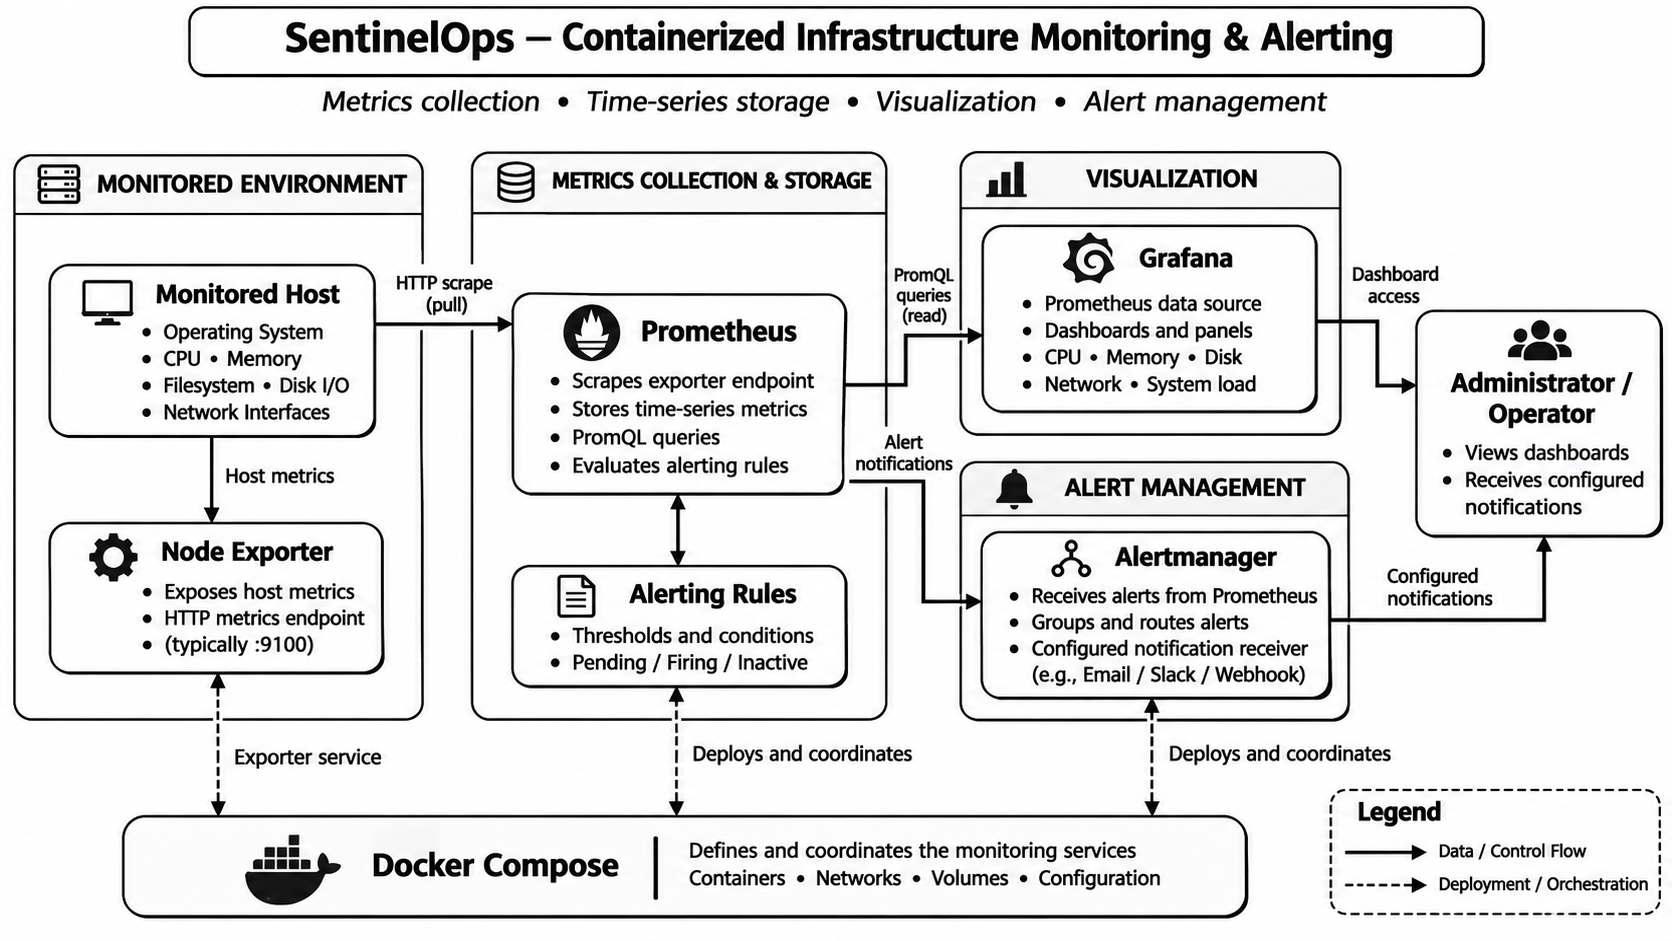
\includegraphics[width=0.98\textwidth]{sentinelops_architecture_bw.png}
\caption{Black-and-white system architecture of the proposed SentinelOps
framework, showing metric collection, visualization, alert management,
and Docker Compose deployment coordination.}
\label{fig:architecture}
\end{figure*}

\subsection{Working Principle}

The monitoring workflow begins when Node Exporter exposes
system-level metrics through its metrics endpoint. Prometheus
periodically accesses this endpoint according to its configured
scrape interval and stores the collected information as
time-series data.

Grafana queries Prometheus to retrieve the required metrics
and displays them through configurable dashboards. These
dashboards allow administrators to observe changes in system
resource utilization.

In parallel, Prometheus evaluates configured alerting rules.
When a condition remains satisfied for its specified duration,
an alert can be generated and forwarded to Alertmanager.
Alertmanager applies the configured grouping and routing
policies to manage the generated alerts.

This workflow provides a centralized approach to monitoring
system performance and identifying potentially critical
resource conditions.

% =================================================
% V. SYSTEM DESIGN AND IMPLEMENTATION
% =================================================

\section{System Design and Implementation}

\subsection{Technology Stack}

SentinelOps is implemented using open-source technologies
that provide metric collection, visualization, alerting,
and containerized deployment.

\begin{table}[!t]
\caption{Technology Stack Used in SentinelOps}
\label{tab:technology}
\centering
\footnotesize
\begin{tabular}{|p{2.0cm}|p{5.0cm}|}
\hline
\textbf{Technology} & \textbf{Purpose} \\
\hline
Prometheus & Metric collection, storage, querying,
and alert evaluation \\
\hline
Node Exporter & Exposes host-level system metrics \\
\hline
Grafana & Dashboard creation and metric visualization \\
\hline
Alertmanager & Alert grouping and routing \\
\hline
Docker Compose & Multi-container deployment and service
coordination \\
\hline
\end{tabular}
\end{table}

\subsection{Metric Collection}

Node Exporter exposes metrics related to the monitored host.
Prometheus is configured to scrape the exporter endpoint
periodically.

The collected metrics provide information about CPU activity,
memory utilization, filesystem capacity, disk operations,
network traffic, and system load.

Prometheus stores these measurements as time-series data,
allowing users to query and analyze resource utilization
over time.

\subsection{Metric Visualization}

Grafana is configured with Prometheus as its data source.
Dashboards provide visual representations of collected
system metrics.

The SentinelOps dashboard includes monitoring panels for:

\begin{itemize}
    \item CPU utilization.
    \item Memory consumption.
    \item Disk usage and disk I/O.
    \item Network traffic and packet activity.
    \item System load.
    \item Process-related information.
\end{itemize}

These visualizations provide an overview of system behaviour
and support the identification of unusual resource utilization
patterns.

\subsection{Alert Configuration}

Prometheus alerting rules are configured to evaluate
selected system metrics against predefined conditions.
These rules can identify conditions such as high CPU
utilization, excessive memory consumption, and high
filesystem usage.

When an alerting condition is satisfied, Prometheus
generates an alert and forwards it to Alertmanager.

Alertmanager manages the received alerts based on its
configuration. Alert grouping and routing help organize
related alerts and direct them to the appropriate notification
receiver.

\subsection{Containerized Deployment}

Docker Compose is used to define and coordinate the monitoring
services. The service configuration specifies the required
containers, port mappings, configuration files, and persistent
storage where configured.

This approach simplifies the startup and management of the
monitoring stack and supports repeatable deployment within
a development environment.

% =================================================
% VI. EXPERIMENTAL SETUP
% =================================================

\section{Experimental Setup}

The SentinelOps framework is implemented and tested in a
containerized development environment. Docker Compose is used
to start and manage the monitoring components.

Prometheus is configured to collect metrics from Node Exporter.
Grafana is connected to Prometheus for dashboard visualization,
while Alertmanager is configured to receive and manage alerts.

\subsection{Monitoring Parameters}

The evaluation considers the following system parameters.

\begin{table}[!t]
\caption{Monitored System Parameters}
\label{tab:metrics}
\centering
\footnotesize
\begin{tabular}{|p{2.0cm}|p{5.0cm}|}
\hline
\textbf{Parameter} & \textbf{Monitoring Purpose} \\
\hline
CPU Utilization & Observes processor activity and usage \\
\hline
Memory Usage & Tracks system memory consumption \\
\hline
Disk Usage & Observes filesystem capacity utilization \\
\hline
Disk I/O & Tracks disk read and write activity \\
\hline
Network Traffic & Observes transmitted and received data \\
\hline
System Load & Provides information about system workload \\
\hline
Process Metrics & Displays process-related system information \\
\hline
\end{tabular}
\end{table}

\subsection{Evaluation Scenarios}

The framework is evaluated through practical monitoring
and alerting scenarios.

\begin{enumerate}
    \item \textbf{Normal Monitoring:} The dashboards are
    observed under normal operating conditions to verify
    metric collection and visualization.

    \item \textbf{Resource Monitoring:} CPU, memory, disk,
    and network metrics are examined through Grafana panels.

    \item \textbf{Alert Evaluation:} Configured Prometheus
    alerting rules are examined to verify their alert states.

    \item \textbf{Alert Management:} Alertmanager is inspected
    to verify the handling and grouping of generated alerts.

    \item \textbf{Recovery Observation:} Alert states are
    observed after the corresponding conditions are no
    longer satisfied.
\end{enumerate}

% =================================================
% VII. RESULTS AND DISCUSSION
% =================================================

\section{Results and Discussion}

The implementation of SentinelOps demonstrates the integration
of metric collection, visualization, and alert management
within a containerized monitoring environment.

\subsection{Dashboard Observations}

The Grafana dashboards provide visual representations of
system-level metrics, including CPU utilization, memory
consumption, disk activity, network traffic, system load,
and process-related information.

The dashboard panels allow users to observe resource
utilization and changes in system behaviour over time.
The integration of Prometheus with Grafana provides a
centralized interface for examining the collected metrics.

\subsection{Alerting Observations}

The configured Prometheus alerting rules are used to
evaluate selected resource conditions. Alerts generated
by Prometheus are forwarded to Alertmanager for management
according to the configured routing policies.

During implementation testing, the alert states were
observed through the Prometheus and Alertmanager interfaces.
The monitoring environment also demonstrated the transition
of alert states as conditions changed.

The observed behaviour indicates that the configured
components can work together to support threshold-based
infrastructure alerting.

\subsection{Qualitative Evaluation}

\begin{table}[!t]
\caption{Observed Functional Evaluation}
\label{tab:results}
\centering
\footnotesize
\begin{tabular}{|p{2.4cm}|p{2.0cm}|p{2.5cm}|}
\hline
\textbf{Test Scenario} & \textbf{Observation} &
\textbf{Evaluation} \\
\hline
Metric Collection & Metrics visible in Prometheus &
Functional \\
\hline
Dashboard Visualization & Monitoring panels displayed in
Grafana & Functional \\
\hline
Alert Rule Evaluation & Alert states visible in Prometheus &
Configured and observed \\
\hline
Alert Management & Alerts handled by Alertmanager &
Configured and observed \\
\hline
Container Deployment & Monitoring services started using
Docker Compose & Functional \\
\hline
\end{tabular}
\end{table}

The functional evaluation demonstrates that SentinelOps
provides an integrated environment for observing system
metrics and managing configured alerts.

However, the evaluation is primarily based on functional
observations. Quantitative performance measurements,
such as metric collection latency, alert delivery time,
and monitoring overhead, are not established in this
version of the study.

% =================================================
% VIII. LIMITATIONS AND FUTURE WORK
% =================================================

\section{Limitations and Future Work}

Although SentinelOps provides an integrated monitoring
environment, several improvements can be considered.

First, the current implementation focuses primarily on
host-level system metrics. Future versions can extend
monitoring to application-level metrics, database
performance, and multiple distributed hosts.

Second, the alerting framework can be enhanced with
additional notification integrations and more advanced
routing policies. This would improve the flexibility
of alert delivery.

Third, the system can be extended with historical
performance analysis and anomaly detection techniques.
Machine learning-based approaches could be explored
to identify unusual resource utilization patterns.

Security improvements, including authentication,
access control, encrypted communication, and secure
secret management, can also be incorporated.

Finally, future evaluation can include quantitative
measurements such as metric collection latency,
alert delivery time, resource overhead, and scalability
under increasing monitoring workloads.

% =================================================
% IX. CONCLUSION
% =================================================

\section{Conclusion}

This paper presented SentinelOps, a containerized
infrastructure monitoring and automated alerting
framework developed using Prometheus, Node Exporter,
Grafana, Alertmanager, and Docker Compose.

The framework integrates system metric collection,
time-series storage, dashboard visualization, and
alert management within a unified environment.
It provides visibility into important system parameters,
including CPU utilization, memory consumption, disk
activity, network traffic, and system load.

The implementation demonstrates how open-source
monitoring technologies can be integrated to simplify
infrastructure observation and support configurable
alerting. Docker Compose further simplifies the
deployment and coordination of the monitoring services.

Future work will focus on extending the framework
towards distributed infrastructure monitoring,
advanced anomaly detection, enhanced notification
mechanisms, security improvements, and quantitative
performance evaluation.

% =================================================
% REFERENCES
% =================================================

\begin{thebibliography}{00}

\bibitem{usman2022}
M. Usman, S. Ferlin, A. Brunstrom, and J. Taheri,
``A Survey on Observability of Distributed Edge \&
Container-Based Microservices,''
\textit{IEEE Access}, vol. 10, pp. 86904--86919, 2022,
doi: 10.1109/ACCESS.2022.3193102.

\bibitem{giamattei2024}
L. Giamattei \textit{et al.},
``Monitoring Tools for DevOps and Microservices:
A Systematic Grey Literature Review,''
\textit{Journal of Systems and Software}, vol. 208,
Art. no. 111906, 2024,
doi: 10.1016/j.jss.2023.111906.

\bibitem{jensen2017}
S. K. Jensen, T. B. Pedersen, and C. Thomsen,
``Time Series Management Systems: A Survey,''
\textit{IEEE Transactions on Knowledge and Data Engineering},
vol. 29, no. 11, pp. 2581--2600, 2017,
doi: 10.1109/TKDE.2017.2740932.

\bibitem{correia2023}
M. Correia, W. Oliveira, and J. Cecilio,
``Monintainer: An orchestration-independent extensible
container-based monitoring solution for large clusters,''
\textit{Journal of Systems Architecture}, vol. 145,
Art. no. 103035, Dec. 2023,
doi: 10.1016/j.sysarc.2023.103035.

\bibitem{pragathi2024}
P. B. C., H. Maddirala, and S. M.,
``Implementing an Effective Infrastructure Monitoring
Solution with Prometheus and Grafana,''
\textit{International Journal of Computer Applications},
vol. 186, no. 38, pp. 7--15, Sep. 2024,
doi: 10.5120/ijca2024923873.

\bibitem{rafiq2025}
M. Rafiq \textit{et al.},
``AI and IoT-Driven Monitoring and Visualisation for
Optimising MSP Operations in Multi-Tenant Networks:
A Modular Approach Using Sensor Data Integration,''
\textit{Sensors}, vol. 25, no. 19, Art. no. 6248, Oct. 2025,
doi: 10.3390/s25196248.

\bibitem{omarbekova2026}
A. O. Omarbekova \textit{et al.},
``Monitoring and Comparative Analysis of Containerized
Environments,'' \textit{Frontiers in Computer Science},
vol. 8, 2026, doi: 10.3389/fcomp.2026.1886850.

\bibitem{prometheus}
Prometheus Authors, ``Prometheus Documentation,''
[Online]. Available:
\url{https://prometheus.io/docs/introduction/overview/}

\bibitem{nodeexporter}
Prometheus Authors, ``Node Exporter,''
Prometheus Exporters Documentation, [Online]. Available:
\url{https://prometheus.io/docs/guides/node-exporter/}

\bibitem{grafana}
Grafana Labs, ``Grafana Documentation,''
[Online]. Available:
\url{https://grafana.com/docs/grafana/latest/}

\bibitem{alerting}
Prometheus Authors, ``Alerting Rules,''
Prometheus Documentation, [Online]. Available:
\url{https://prometheus.io/docs/prometheus/latest/configuration/alerting_rules/}

\bibitem{alertmanager}
Prometheus Authors, ``Alertmanager Documentation,''
[Online]. Available:
\url{https://prometheus.io/docs/alerting/latest/alertmanager/}

\bibitem{dockercompose}
Docker Inc., ``Docker Compose Documentation,''
[Online]. Available:
\url{https://docs.docker.com/compose/}

\end{thebibliography}

\end{document}
